\documentclass[titlepage,12pt]{article}
\usepackage[margin=1in]{geometry}
\usepackage[inline]{enumitem}
\usepackage{titlesec}
\usepackage{textcomp}
\usepackage{amsmath}
\usepackage{graphicx}
\usepackage[pdftex]{hyperref}
\usepackage[english]{babel}
\usepackage{csquotes}
\usepackage{titling}
\usepackage{titlesec}
\usepackage{xspace}
\usepackage{tabularx}
\usepackage{float}
\usepackage{parskip}
\usepackage{blindtext}
\usepackage{listings}
\usepackage{minted}

\MakeOuterQuote{"}

\setminted{autogobble,python3,mathescape,fontsize=\footnotesize}
\newcommand\tab[1][.5in]{\hspace*{#1}}
\newcommand\name{VRsh}

\title{Final Project Design v. 1.1}
\author{Sumner Evans, Robbie Merillat, Sam Sartor}
\date{\today}

\begin{document}

\maketitle

\section{Design History}
\begin{tabularx}{\linewidth}{| l | l || X |}
    \hline
    \textbf{Version Number} & \textbf{Date} & \textbf{Change Description} \\
    \hline\hline
    1.0 & 2017--11--07 & First Draft \\
    \hline
    1.1 & 2017--11--15 & Second Draft \\
    \hline
\end{tabularx}

\section{Overview}
VR Technology has been developing rapidly in the 21st century. Current solutions
such as Unity attempt to use old programming languages and paradigms to
implement VR environments and thus limit developers' abilities to create new and
unique environments. With every cutting edge technology, new paradigms and
design patterns must be invented. This project intends to explore and implement
these paradigms and design patterns.

For this project, we will utilize a 3D space to implement an intuitive UI for
\begin{enumerate*}[label={(\alph*)}]
    \item loading programs,
    \item saving program state, and
    \item customizing the environment
\end{enumerate*} (described in Section~\ref{sec:design}).  We believe that
implementing a shell-like environment is the most effective method for us to
explore those patterns.

\section{Design}\label{sec:design}
There are three main goals for our project (referred to as \textit{\name} for
now):
\begin{enumerate}
    \item \textbf{Loading Programs:} the user will be able to load our three
        individual programs from our {\name} as described in Section~\ref{sec:ui}.
    \item \textbf{Saving Program State:} the user will be able to save the state
        of an environment (program). This is elaborated in
        Section~\ref{sec:state}.
    \item \textbf{Customizing the Environment:} the user will be able to
        customize the {\name} environment. See Section~\ref{sec:env} for details.
\end{enumerate}

\subsection{Visual Design}
The visual design of this program is dynamic in that both the general
settings and environment can be modified. This would look and feel
similar to the Steam VR personal "desktop" with added options for settings
and environment customization. "Running" a program will switch from the {\name}
home environment to the desired program environment.

\subsubsection{Global UI}\label{sec:ui}
There will be a persistent user interface that will be visible from the {\name}
home environment and from within the individual environments that can be
accessed from within \name. This UI will be a ``halo'' centered at the user,
located above the user's head. The halo will have components attached to allow
the user to perform actions such as running programs and moving between
environments. We have not yet determined the most intuitive design motif for
these controls. However, we have brainstormed a few innovative ideas for these
controls including grab-and-pull-down selectors, Rolodex selectors, and system
setting asteroid field of options. Some of these concepts can bee visualized in
the image below.

\begin{center}
    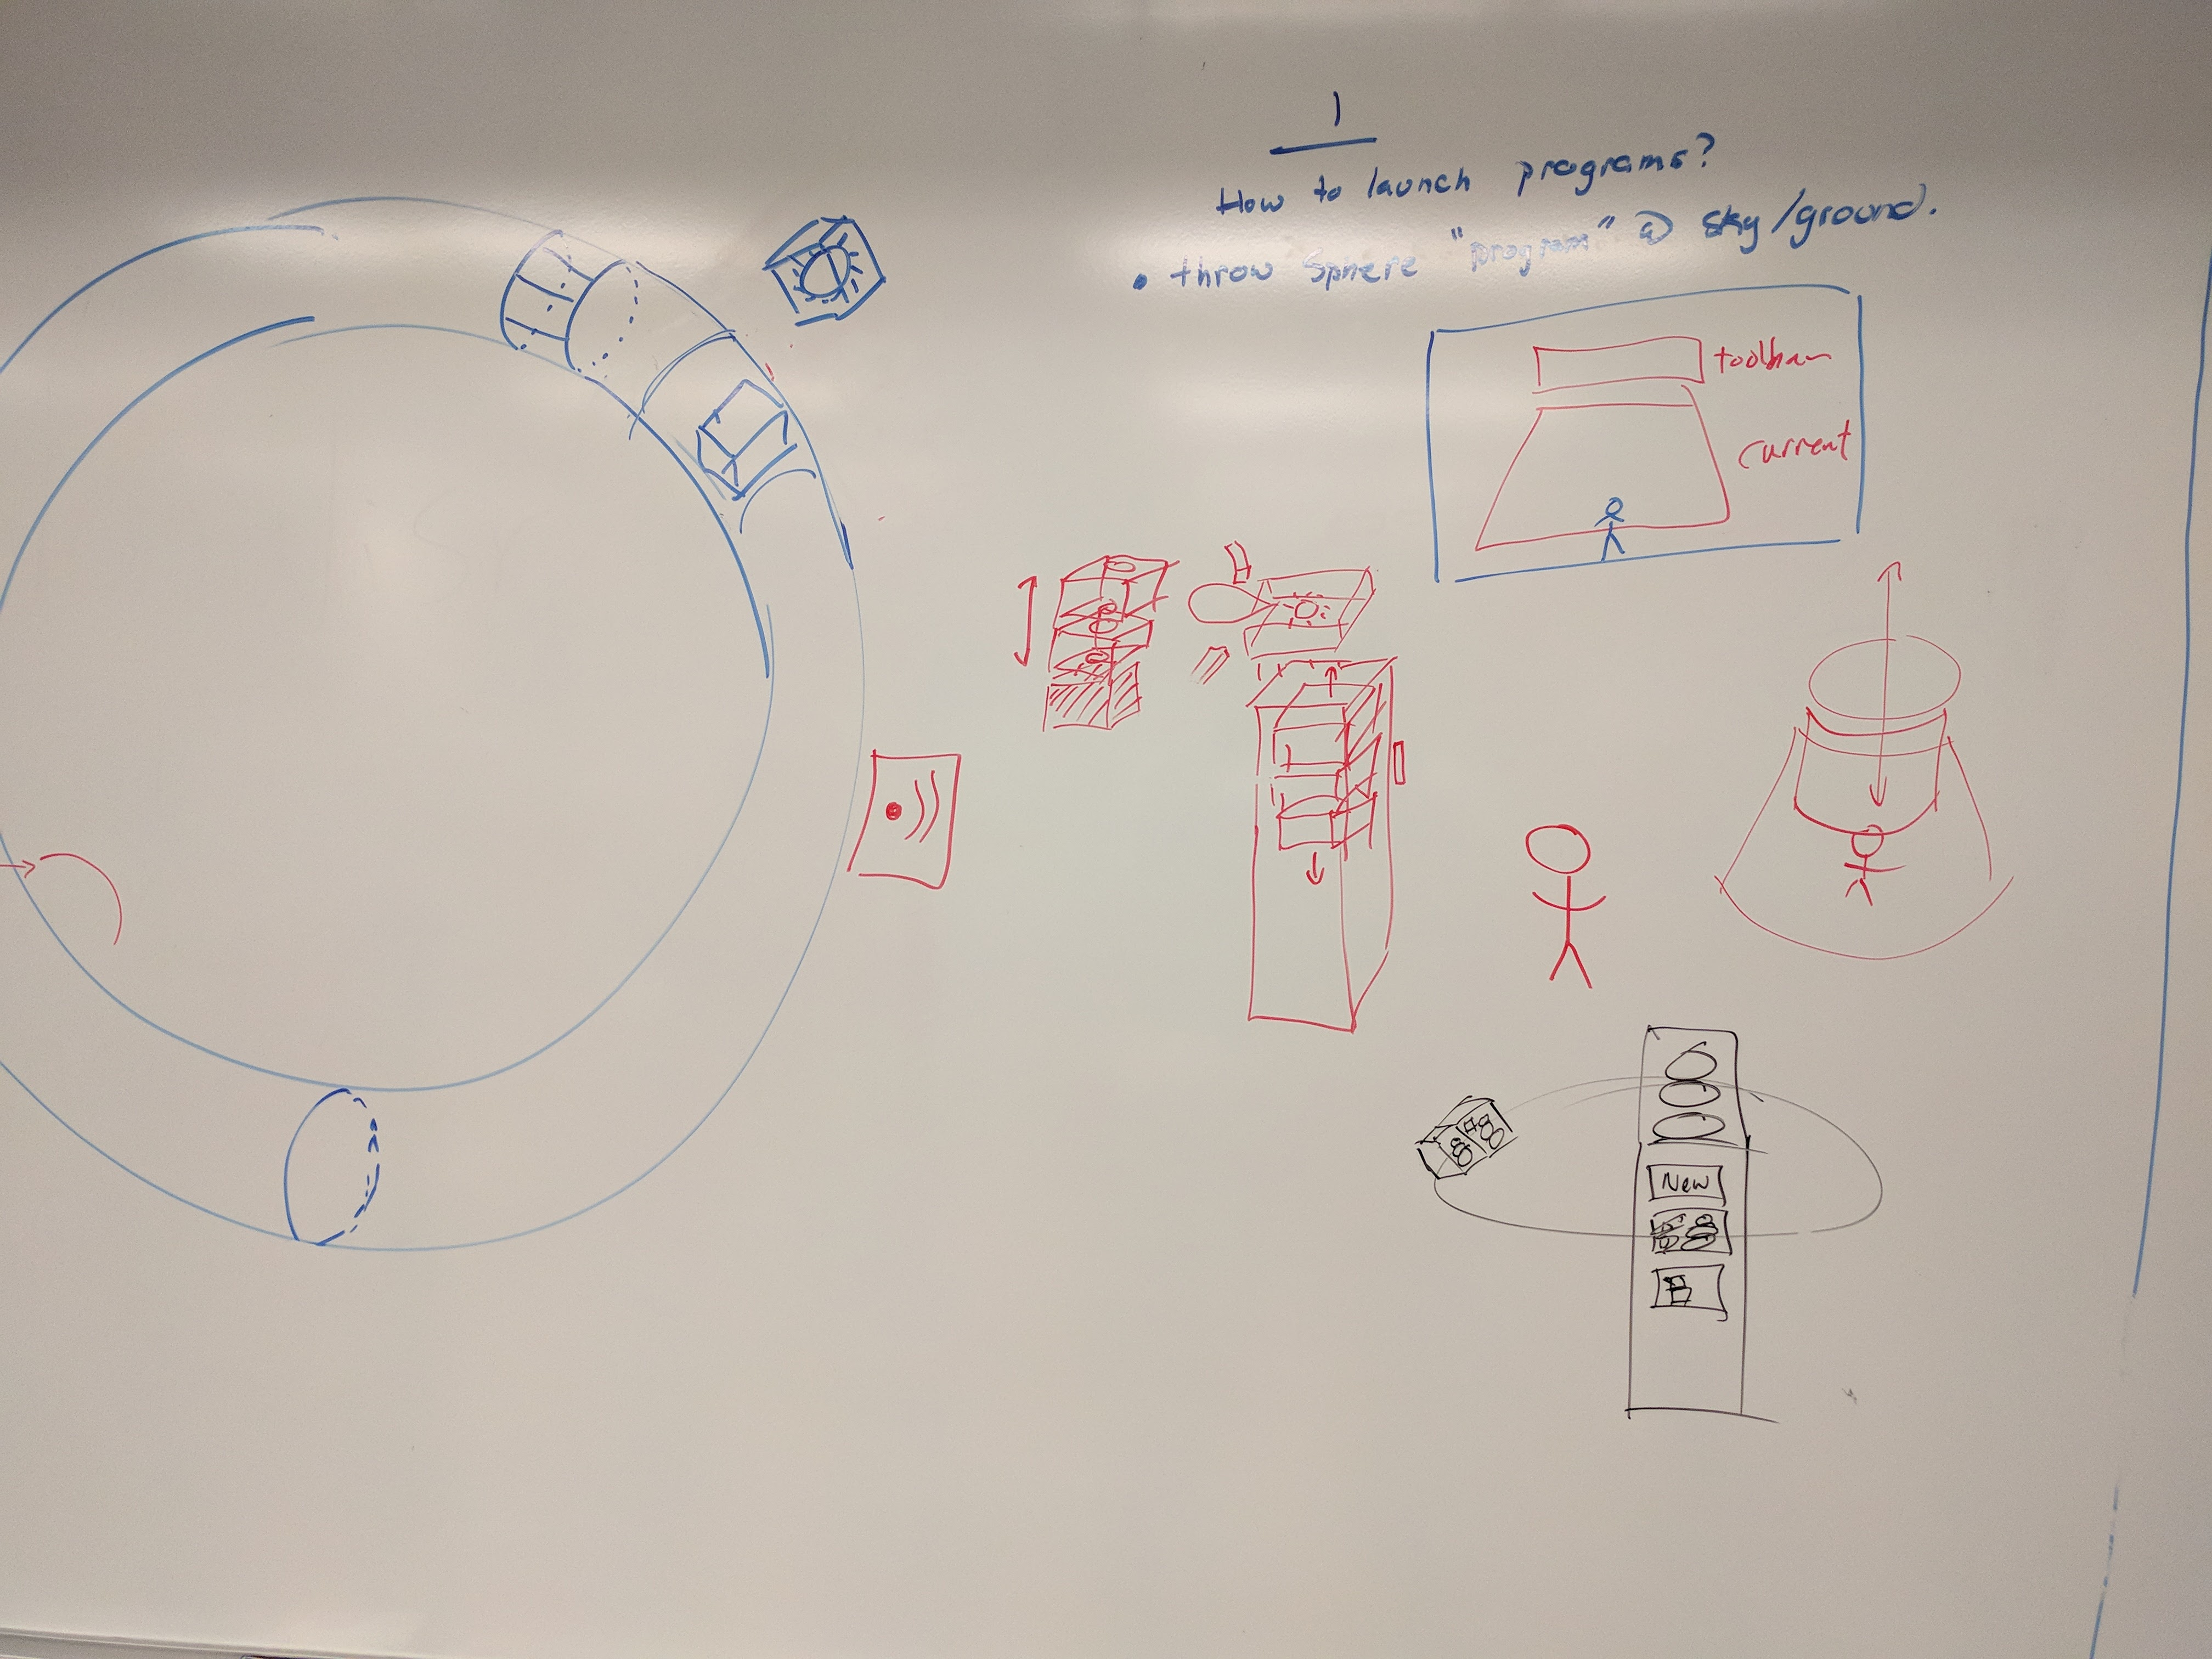
\includegraphics[width=0.8\textwidth]{./images/visual.jpg}
\end{center}

\subsubsection{Customizable Environment}\label{sec:env}
Several components will enable the user to customize their {\name} home
environment. Mentioned above, the system setting asteroid field will
allow the user to create a new entity within their home environment.
Some entities may last for a set amount of time without being interacted
with, while others remain persistent. Examples of these entities could be:
\begin{itemize}
    \item Brightness Bar: changes ambient brightness
    \item Skymap Texture: Throw to apply image as background
    \item Color Wheel: modify colors
    \item Mode: sitting vs.\ standing modes
    \item Various Objects: place objects around the home environment, allowing
        customization
        \begin{itemize}
            \item Clouds/Mist
            \item Boxes
            \item Penguin
            \item Mjolnir
            \item Rugs
            \item Plushes
            \item Weapons (Pikes, Axes, Swords, Bow/Arrow)
        \end{itemize}
\end{itemize}

\subsubsection{Interactions}

Interactions will include:
\begin{itemize}
    \item Object surface/node snapping
    \item A yank control to bring objects closer/further
    \item Grabbing an object at a point
    \item Throwing objects (grab maintains momentum)
    \item Expanding fixed menus
    \item Applying tool objects to other objects
    \item Inter-object collisions
\end{itemize}

\subsubsection{Lighting Model} We have several lighting/rendering models
available, however most assets will use physically based rendering.

\subsection{System State Storage}\label{sec:state}
To facilitate the storage of environment state, {\name} will create a directory
in the \texttt{.config} folder of the user's home directory called
\texttt{\MakeLowercase\name} and store all necessary information in that
directory.

\newpage
Our preliminary folder structure is as follows:
\begin{minted}{html}
.vrsh
|-> environments                        // all environment state data
|   |-> home                            // for the savefiles
|   |   |-> 2017-11-14-172312.save      // data format of these files can be
|   |   |-> 2017-11-14-173708.save      // determined by the program that is
|   |   |-> 2017-11-14-184937.save      // associated with this environment
|   |   |-> ...
|   |-> snowflakes
|   |   |-> 2017-11-14-172312.save
|   |   |-> 2017-11-14-173708.save
|   |   |-> 2017-11-14-184937.save
|   |   |-> ...
|   |-> lets-get-physical
|   |   |-> 2017-11-14-172312.save
|   |   |-> 2017-11-14-173708.save
|   |   |-> 2017-11-14-184937.save
|   |   |-> ...
|   |-> workbench
|-> config                              // for general configs (if necessary)
\end{minted}

Individual programs are responsible for
\begin{enumerate*}[label={(\alph*)}]
\item opening these environments,
\item creating 3D ``thumbnails'' for the environments, and
\item creating the file's binary data
\end{enumerate*}.

\section{Management}

\subsection{Project Scope}
Our original goal was to implement a fully featured Linux shell that is able to
wrap Linux commands in a VR environment. We realized that this was infeasible
with our limited experience with VR and quickly changed the scope. At this
point, we have created an achievable and measurable plan to implement the
features that we want to include in the final project. Our plan consists of
three milestones (see Table~\ref{tab:milestones}) with specific goals.

\begin{table}[H]
    \caption{Milestone Delivery Schedule}\label{tab:milestones}
    \centering
    \begin{tabular}{|p{12cm}|l|}
        \hline
        \textbf{Milestone} & \textbf{Date} \\
        \hline\hline
        Milestone I:\ Design Document & 2017/11/08 \\
        \hline
        Milestone II:\ Individual Project Program Picking (Demo) & 2017/11/27 \\
        \hline
        Milestone III:\ Final Code Submission
        \begin{itemize}
            \item Individual project improvements
            \item Saving Program State
            \item Customizable home environment
        \end{itemize} & 2017/12/13\\
        \hline
    \end{tabular}
\end{table}

\subsection{Risk Analysis}
While we have done a significant amount of brainstorming and design work for our
{\name} environment, we have not begun to implement any of the environment.
This is a large risk for us, as there will be many unanticipated problems which
may alter the complexity of our goals. Scope creep is another risk for our team,
as a few of us are notorious for adding unnecessary features to our
applications.

Currently, we have a decent idea of how to store state, however, we have not
begun to implement it. This is another major risk for us. Another risk that we
must mitigate is settling for less than what our goals because of deadlines. To
counter this, we will will be proactive with scheduling to help ensure that we
meet our goals.

Our dependency tree is relatively thick, so our code is vulnerable to external
dependency disruption making the cost of refactoring high.

\subsection{Test Plan}
We will have an appropriate number of unit tests in our code, especially our
libraries (\texttt{flight} and \texttt{picea}). Additionally, we plan to iterate
quickly on the program, testing as we develop to help ensure that program
behaves as predicted.

\subsection{Demo Plan}
We will be demoing our intermediate milestones during our meetings. Our goal is
to have this project ready for the C-MAPP event on January 18, 2018.

\section{Dependencies}
These are the libraries that we are using in our application. Dependencies
marked with a \texttt{*} are made by this team.
\begin{table}[H]
    \caption{Dependency List}\label{tab:milestones}
    \centering
    \begin{tabular}{|l|p{12cm}|}
        \hline
        \textbf{Dependency} & \textbf{Purpose} \\
        \hline
        \hline
        \texttt{flight*} & Rendering, graphical user interface, asset loading,
            and VR hardware library \\
        \hline
        \texttt{picea*} & Dynamic, event-oriented object trees \\
        \hline
        \texttt{serde} & Data serialization and deserialization \\
        \hline
        \texttt{nphysics} & Physics engine \\
        \hline
        \texttt{ncollide} & Vector and matrix math \\
        \hline
        \texttt{nalgebra} & Geometric/volumetric operations and queries \\
        \hline
    \end{tabular}
\end{table}

\end{document}
